%%%% acra.tex

\typeout{ACRA Instructions for Authors}

% This is the instructions for authors for ACRA.
\documentclass{article}
\usepackage{acra}
\usepackage{lmodern}% http://ctan.org/pkg/lm
\usepackage{amsmath}
\usepackage{graphicx}
\usepackage{color}
\usepackage{hyperref}
\usepackage{amssymb}
\usepackage{url}
\usepackage{pdfpages}
\usepackage{fancyhdr}
\usepackage{subfig}
\usepackage{listings} 
\usepackage{selinput}    

% The file acra.sty is the style file for ACRA. 
% The file named.sty contains macros for named citations as produced 
% by named.bst.

% The preparation of these files was supported by Schlumberger Palo Alto
% Research, AT\&T Bell Laboratories, and Morgan Kaufmann Publishers.
% Shirley Jowell, of Morgan Kaufmann Publishers, and Peter F.
% Patel-Schneider, of AT\&T Bell Laboratories collaborated on their
% preparation. 

% These instructions can be modified and used in other conferences as long
% as credit to the authors and supporting agencies is retained, this notice
% is not changed, and further modification or reuse is not restricted.
% Neither Shirley Jowell nor Peter F. Patel-Schneider can be listed as
% contacts for providing assistance without their prior permission.

% To use for other conferences, change references to files and the
% conference appropriate and use other authors, contacts, publishers, and
% organizations.
% Also change the deadline and address for returning papers and the length and
% page charge instructions.
% Put where the files are available in the appropriate places.

\title{Kalman filter to solve a Linear Dynamical System}
\author{Diego Garrido}

\begin{document}

\maketitle
\href{https://nbviewer.jupyter.org/github/dgarridoa/Kalman_Filter/blob/master/Kalman_Filter.ipynb}{\color{blue}{Jupyter Notebook}}
\section{Introduction}

A state space model or SSM can be written in the following generic form:

\begin{align}
z_{t} = g(u_{t}, z_{t-1}, \epsilon_{t})\\
y_{t} = h(z_{t}, u_{t}, \delta_{t})
\end{align}

where $z_{t}$ is the hidden state, $u_{t}$ is an optional input or control signal, $y_{t}$ is the observation, $g$ is the transition model, $h$ is the observation model, $e_{t}$ is the system noise at time $t$, and $\delta_{t}$ is the observation noise at time $t$. The primary goals in using SSMs is to recursively estimate the belief state, $p(z_{t}|y_{1:t}, u_{1:t}, \theta)$, where $\theta$ are the parameters of the model and is known.

An important special case of an SSM is where all the CPDs are linear-Gaussians. In other words, we assume:

\begin{align}
\centering
\mu_{t,t-1} & \triangleq A_{t}\mu_{t-1}+B_{t}u_{t}\\
\Sigma_{t,t-1} & \triangleq A_{t}\Sigma_{t-1}A_{t}^{T}+Q_{t}\\
z_{t} &= A_{t}z_{t-1}+B_{t}u_{t}+\epsilon_{t}\\
y_{t} &= C_{t}z_{t}+D_{t}u_{t}+\delta_{t}\\
e_{t} &\sim \mathcal{N}(0, Q_{t})\\
\delta_{t} &\sim \mathcal{N}(0, R_{t})
\end{align}

This model is called a linear-Gaussian SSM (LG-SSM) or a linear dynamical system (LDS). If the parameters $\delta_{t} = (A_{t}, B_{t}, C_{t}, D_{t}, Q_{t}, R_{t})$ are independent of time, the model is called stationary. In this case we can estimate the posterior mean and covariance of the hidden variable using the Kalman filter where:

\begin{align}
    \centering
    \mu_{t,t-1} & \triangleq A_{t}\mu_{t-1}+B_{t}u_{t}\\
    \Sigma_{t,t-1} & \triangleq A_{t}\Sigma_{t-1}A_{t}^{T}+Q_{t}\\
    r_{t} &\triangleq y_{t}-\hat{y}_{t}\\
    \hat{y}_{t} &\triangleq  C_{t}\mu_{t|t-1}+D_{t}u_{t}\\
    K_{t}  &\triangleq \Sigma_{t|t-1}C_{t}^{T}S_{t}^{-1}\\
    S_{t}  &\triangleq  C_{t}\Sigma_{t|t-1}C_{t}^{T}+R_{t}\\
    \mu_{t} & = \mu_{t|t-1}+K_{t}r_{t}\\
    \Sigma_{t} & = (I-K_{t}C_{t})\Sigma_{t|t-1} 
\end{align}

\section{Implementation}
Consider an object to a constant velocity in a 2D plane, let $z \in \mathbb{R}^{4}$ the vector with the positions and velocities and $y \in \mathbb{R}^{2}$ the observed location of the object. Our ``best guess" about the location of the object is the posterior mean, denoted as a red cross in Figure 1. Our uncertainty associated with this is represented as an ellipse, which contains 95\% of the probability mass. We see that out uncertainty fall down over time, as the effects of the initial uncertainty. We also see that the estimated trajectory has ``filtered out" some of the noise.


\begin{figure}[h]
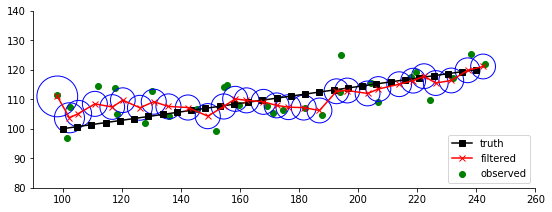
\includegraphics[scale=0.4]{kalman_filter.png}
\caption{Illustration of Kalman filtering. Ground truth (black squares) are generated by an object moving in a 2D plane to a constant velocity. Observations (green circles) are generated by applying Gaussian noise to the ground truth. Red cross is the posterior mean, blue circles are 95\% confidence ellipses derived from the posterior covariance.}
\end{figure}


\end{document}